\documentclass[10pt, letterpaper]{article}
\usepackage{mathtools}
\usepackage{amsmath}
\usepackage[margin=0.5in]{geometry}
\usepackage{graphicx}
\graphicspath{ {./images/} }
\setcounter{MaxMatrixCols}{12}
\renewcommand{\thesubsection}{\alph{subsection}}
\begin{document}

\title{Adv Controls HW 2}
\author{Daniel Wood}
\maketitle
\section{Problem 1}

\subsection{.)}

\[
x = \left[\begin{matrix}
\alpha\\
\dot{\alpha}\\
\theta\\
\dot{\theta}\end{matrix}\right]
\]

\[
\dot{x} = f(x) + g(x)\tau
\]

where,

\[
f(x) = \left[\begin{matrix}
\dot{\alpha}\\
\frac{B_{m} \dot{\theta} r {cos}(\alpha) + J_{b} \dot{\alpha}^{2} l_{p} {sin}(\alpha) {cos}(\alpha) + J_{b} g {sin}(\alpha) + \dot{\alpha}^{2} l_{p}^{3} m_{p} {sin}^{2}(\alpha) {cos}(\alpha) + \dot{\alpha} \dot{\theta} l_{p}^{2} m_{p} r {cos}^{2}(\alpha) + g l_{p}^{2} m_{p} {sin}^{2}(\alpha) + g m_{p} r^{2} {sin}(\alpha)}{J_{b} l_{p} + l_{p}^{3} m_{p} {sin}(\alpha) + l_{p} m_{p} r^{2} {sin}^{2}(\alpha)}\\
\dot{\theta}\\
\frac{- B_{m} \dot{\theta} + \dot{\alpha}^{2} l_{p} m_{p} r {sin}^{3}(\alpha) - \dot{\alpha} \dot{\theta} l_{p}^{2} m_{p} {cos}(\alpha) - g m_{p} r {sin}(\alpha) {cos}(\alpha)}{J_{b} + l_{p}^{2} m_{p} {sin}(\alpha) + m_{p} r^{2} {sin}^{2}(\alpha)}\end{matrix}\right]
\]

\[
g(x, \tau) = \left[\begin{matrix}
0\\
- \frac{r {cos}(\alpha)}{J_{b} l_{p} + l_{p}^{3} m_{p} {sin}(\alpha) + l_{p} m_{p} r^{2} {sin}^{2}(\alpha)}\\
0\\
\frac{1}{J_{b} + l_{p}^{2} m_{p} {sin}(\alpha) + m_{p} r^{2} {sin}^{2}(\alpha)}\end{matrix}\right]\tau
\]

\subsection{.)}

\[
y = \left[\begin{matrix}
1 & 0 & 0 & 0\end{matrix}\right]
\left[\begin{matrix}
\alpha\\
\dot{\alpha}\\
\theta\\
\dot{\theta}\end{matrix}\right] = \alpha
\]

\[
\frac{dy}{dt} = \dot{\alpha}
\]

\[
\frac{d^{2}y}{dt^{2}} = \ddot{\alpha} = f(\tau)
\]

Thus relative degree of 2.

\subsection{.)}

Because of relative degree of 2, a transformation can be defined as:

\[
T = \left[\begin{matrix}
\phi(x)\\
L^{0}_{f}h(x)\\
L^{1}_{f}h(x)
\end{matrix}\right]
=
\left[\begin{matrix}
\eta\\
\xi_{1}\\
\xi_{2}
\end{matrix}\right]
\]

\[
\xi_{1} = L^{0}_{f}h(x) = \alpha
\]

\[
\xi_{2} = L^{1}_{f}h(x) = \dot{\alpha}
\]

\[
\frac{\partial{\phi(x)}}{\partial{x}}G(x, \tau) = 0
\]

substituting $G(x, \tau)$:

\[
\frac{\partial{\phi(x)}}{\partial{\alpha}}[- \frac{\tau r {cos}(\alpha)}{J_{b} l_{p} + l_{p}^{3} m_{p} {sin}(\alpha) + l_{p} m_{p} r^{2} {sin}^{2}(\alpha)}] + 
\frac{\partial{\phi(x)}}{\partial{\theta}}[\frac{\tau}{J_{b} + l_{p}^{2} m_{p} {sin}(\alpha) + m_{p} r^{2} {sin}^{2}(\alpha)}] = 0
\]

\[
\frac{\partial{\phi(x)}}{\partial{\alpha}} + \frac{-\tau(J_{b} l_{p} + l_{p}^{3} m_{p} {sin}(\alpha) + l_{p} m_{p} r^{2} {sin}^{2}(\alpha))}{\tau r {cos}(\alpha)(J_{b} + l_{p}^{2} m_{p} {sin}(\alpha) + m_{p} r^{2} {sin}^{2}(\alpha))}\frac{\partial{\phi(x)}}{\partial{\theta}} = 0
\]

\[
\frac{\partial{\phi(x)}}{\partial{\alpha}} + \frac{-l_{p}}{r {cos}(\alpha)}\frac{\partial{\phi(x)}}{\partial{\theta}} = 0
\]

separation of variables and solving yields:

\[
\phi(x) = -\theta + \frac{r}{l_p}{sin}(\alpha) = \eta
\]

taking the derivative:

\[
\dot{\eta} = -\dot{\theta} + \frac{r}{l_p}{cos}(\alpha)\dot{\alpha}
\]

substituting for $\dot{\alpha}$, $\dot{\theta}$

\[
\dot{\eta} = -\dot{\theta} + \frac{r}{l_p}{cos}(\xi_{1})\xi_{2}
\]

then,

\[
\dot{\xi_{1}} = \xi_{2}
\]

\[
\dot{\xi_{2}} = 
\]

\[
y = \xi_{1}
\]

\section{Problem 2}

\subsection{.)}

\begin{figure}[h]
\caption{Phase Portraits, Predator vs. Prey}
\centering
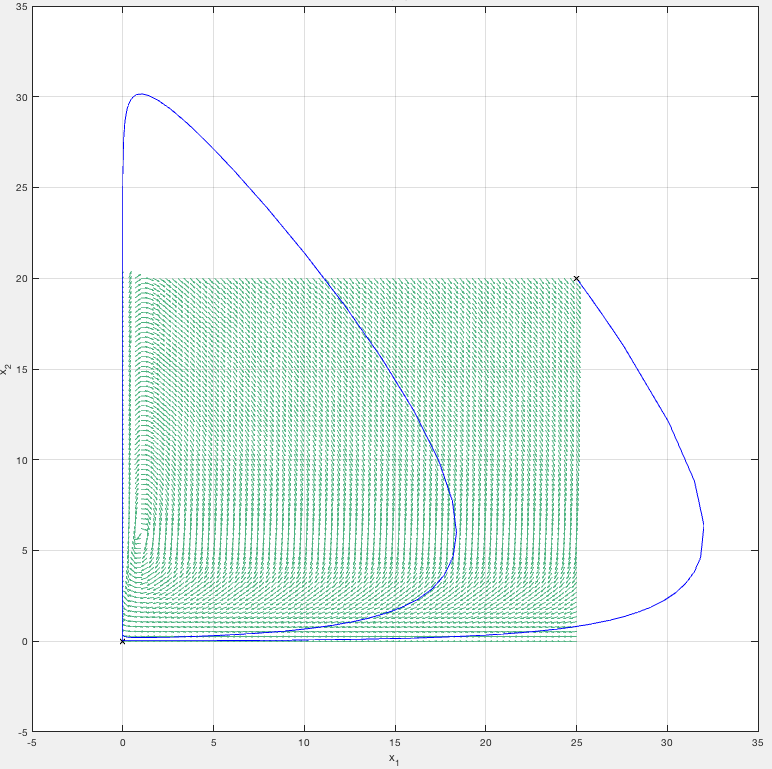
\includegraphics[scale=0.3]{HW2_2}
\end{figure}

\subsection{.)}

\[
f(x) = \left[\begin{matrix}
x_{1}x_{2} - 4x_{1}\\
-x_{1}x_{2} + 2x_{2}
\end{matrix}\right]
\]

\[
g(x) = \left[\begin{matrix}
-2x_{1}\\
-x_{2}
\end{matrix}\right]
\]

\[
\dot{S} = 2x_{1}\dot{x_{1}} + 2x_{2}\dot{x_{2}} - 20\dot{x_{1}} - 20\dot{x_{2}}
\]

substituting $\dot{x_{1}}$, $\dot{x_{2}}$:

\[
\dot{S} = 2x_{1}^{2}x_{2} - 8x_{1}^{2}-4x_{1}^{2}u -2x_{1}x_{2}^{2} + 4x_{2}^{2} -2x_{2}^{2}u + 80x_{1} + 40x_{1}u-40x_{2}+20x_{2}u < 0
\]

\[
\dot{S} = 2x_{1}^{2}x_{2} - 8x_{1}^{2}-4x_{1}^{2}u -2x_{1}x_{2}^{2} + 4x_{2}^{2} -2x_{2}^{2}u + 80x_{1} + 40x_{1}u-40x_{2}+20x_{2}u > 0
\]

and,


\[ u(x) = \begin{cases} 
      [\frac{2x_{1}^{2}x_{2} - 8x_{1}^{2}-2x_{1}x_{2}^{2} + 4x_{2}^{2} + 80x_{1}-40x_{2}}{-4x_{1}^{2}-2x_{2}^{2}+40x_{1}+20x_{2}}] & s(x) > 0\\
      -[\frac{2x_{1}^{2}x_{2} - 8x_{1}^{2}-2x_{1}x_{2}^{2} + 4x_{2}^{2} + 80x_{1}-40x_{2}}{-4x_{1}^{2}-2x_{2}^{2}+40x_{1}+20x_{2}}] & s(x) < 0\\
   \end{cases}
\]

\end{document}